\section{Interpolation}

Digital delay lines are implemented using a memory buffer of discrete audio samples. To change the delay time, we change the distance in the buffer between where samples are written and where they are read back.\cite{reiss2014audio}
It is often necessary for a delay line to vary in length. Usually, separate read and write pointers are used. Additionally, for good quality audio, it is necessary to interpolate the delay-line length rather than ``jumping'' between integer numbers of samples. This is typically accomplished using an interpolating read to make the delay line vary smoothly over time.~\cite{smith2010physical}
In our work we tried implementing both linear interpolation and 2ndorder polynomial interpolation and the second one seemed to be the smoother one.

\paragraph{Linear Interpolation}
Linear interpolation is the most commonly used case because it is easy to implement and inexpensive.
It works by effectively drawing a straight line between two neighboring samples and returning the appropriate point along that line (see ~\ref{fig:linear-interpolation}).
  
\begin{figure}[h]
	\centering
  	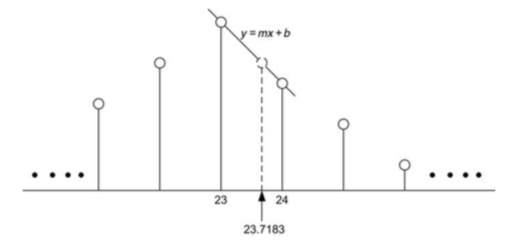
\includegraphics[width=0.8\linewidth]{assets/Linear interpolation of sample values.png}
  	\caption{Linear interpolation of sample values}
  	\label{fig:linear-interpolation}
\end{figure}



\paragraph{Polynomial Interpolation}
In polynomial interpolation a curve is drawn between the points (or a series of points), and then the interpolated value is found on that curve.~\cite{pirkle2013designing}



